% !TEX root = ../main.tex
\chapter{阿尔茨海默症的智能辅助分类} 
\label{chapter:fineClassify}
当前神经网络驱动的图像分类算法普遍存在仅能捕获局部空间特征的问题,这在一定程度上制约了特征抽取的有效性,进而可能影响到分类性能的整体准确性。特别是在AD早期阶段的诊断分类任务中,面对从EMCI、MCI到LMCI这一连续进展阶段的精细化分类任务,亟需发展更加稳健且智能的分类策略,以实现对疾病进程的精准评估与预测。
在这一章中,将介绍一种以影像为导向的新小波卷积单元神经网络。一方面,为了获得非局部的感受野以及避免信息丢失,本章定义了一个新的卷积运算单元。使用该小波卷积单元,进一步设计了一个基于它的细粒度AD多分类网络\cite{wen2023fine},在细粒度多分类任务上实现了更高的分类精度。
%到目前为止,只有少数方法研究了一种或多种AD的细粒度分类,能够同时实现细粒度和多类分类的方法更少。本章采用了新的网络在DTI影像上实现细粒度分类,达到了较先进的水平。
%,实验得到的八种细粒度分类的准确率分别为97.30\%,95.78\%,95.00\%,94.00\%,97.89\%,95.71\%,95.07\%,93.79\%。
%为了建立AD分类的参考标准,本章实现了所有粗粒度和细粒度的12种分类。结果表明,本章提出的方法实现了更高的分类精度。

\section{引言}
AD是在老年人群中非常常见的一种疾病。目前,还没有有效的治疗方法可以治愈AD或改变其进展。MCI是介于AD和NC之间的中间阶段。临床研究表明,MCI可分为EMCI和LMCI。EMCI阶段是可逆的,及时发现和干预可以避免AD的发展,而在LMCI阶段及时诊断和治疗可以延缓AD的发展或治愈AD,因此痴呆的早期发现和诊断将成为主要目标。AD的早期准确诊断是一个有意义和挑战性的任务。


卷积神经网络在非医疗影像分类领域取得了显著成效,因此众多研究开始探索将其技术应用于医学影像分类以及智能化辅助疾病的诊断。尤其是在过去的十年间,学者们提出了一系列基于深度学习技术针对AD分类的方法,如表\ref{paper3accuracy1}所示。但同时,这些现有方法也暴露出一些局限性问题。
\begin{itemize}
    \item 当前大多数运用深度学习技术对AD进行分类的方法,通常采用的是为非医学影像设计的标准卷积操作,其局限性在于局部感受野受限。尽管空洞卷积能有效拓宽局部感知范围,但同时也会导致大量信息的丢失问题。与自然图像不同,整个医学影像中的细节特征都比较重要。另外,细粒度AD分类的实现和准确性面临着一定的挑战和瓶颈。为了更有效地提取医学影像的深度特征,需要一种新的非局部感受野卷积运算。
    \item 现有的大多数AD分类方法只能实现粗粒度的分类。只有少数方法,例如\cite{Fangmeie2022,de2021dti},研究了某些类型的细粒度分类,而细粒度的分类具有更重要的临床意义。此外,AD分类方法很多,但它们所能实现的分类组合参差不齐。需要一种能够实现12种全分类的方法,为该领域的研究提供参考。
    \item 大多数现有的工作采用MRI数据进行AD分类。根据临床医学理论,DTI反映了脑内纤维束间组织结构的连续性,与AD密切相关。因此,本章选择DTI进行细粒度的AD分类。
\end{itemize}

关于DTI数据的选择,本章给予以下详细的解释。神经影像学检查的方式(包括DTI扫描、正电子发射断层扫描(PET)扫描、MRI扫描等)通常用于AD的诊断。DTI\cite{huynh2019multi}也称为基于水分子运动的特殊MRI模态。DTI成像的原理是水分子在梯度场中的扩散改变磁矩。因此,这项创新技术能够清晰展示大脑白质区域中神经束的布局,以揭示人体中枢神经系统的纤维构造细节。脑中纤维束之间组织结构的连续性可以从水中扩散纤维束的成像中推断\cite{frisoni2010clinical}。在AD患者的研究中,DTI影像显示为灰质、白质等的FA(各向异性分数)异常降低和MD(平均扩散率)值异常增加。因此,与其他影像数据相比,DTI数据更有利于实现早期的细粒度分类。

为了突破现有AD分类方法的上述局限性,本章将小波理论应用于卷积运算中,定义了一种新的卷积单元,并将单尺度和多尺度小波分解的特征融合在一起,以获得非局部的感受野,避免信息丢失。采用新的小波卷积单元(wavelet convolution unit,WCU),本章基于DTI数据实现了12种所有组合分类,特别是对于细粒度分类,提高了分类精度。
总之,本章提出了一个小波卷积单元来构建一个有效的WCU网络,用于细粒度和多AD分类。使用WCU的深度学习方法和DTI数据主要证明本章提出的方法实现了更高精度的细粒度AD分类。
本节工作的三个主要创新点:
\begin{itemize}
    \item 本章提出了一种新的卷积单元(WCU),将小波变换与传统的卷积函数相结合,以获得非局部的感受野,避免信息丢失。嵌入WCU的网络大大提高了卷积神经网络的性能。WCU是首个将小波分析嵌入到初级的卷积神经网络中的智能辅助阿尔茨海默症分类的工作。
    \item 本章提出了一种基于WCU和脑影像DTI数据的AD分类网络框架(WCU-Net)。首次实现了所有粗粒度和细粒度的组合分类。大多数现有的AD分类方法限于AD与MCI与NC之间的粗粒度分类,少数方法实现了一种或几种细粒度分类。本章所提出的方法实现了所有八种细粒度分类,其中,首次出现细粒度三分类。该方法为以后的AD分类研究提供了参考标准。
    \item 本章的工作实现的所有12种分类获得了高准确率,特别是对8种细粒度分类的准确率从92.5\%,92.6\%,93.5\%,90.9\%,81\%,无,无,92.6\%提高到97.30\%,95.78\%,95.00\%,94.00\%,97.89\%,95.71\%,95.07\%,93.79\%。首先,提出了细粒度的三分类方法,准确率达到95\%以上。细粒度二分类EMCI与LMCI相比,分类准确率提高了16.89\%。细粒度四分类的准确率达到93.79\%,比现有方法提高了1.19\%。此外,通过使用来自合适的预训练经典网络模型的初始权重,可以进一步提高准确性。
\end{itemize}


\ref{chapter4.2}节简要介绍了包括小波分析在内的频域分析方法及其在图像处理中的应用,并介绍了基于神经网络的AD辅助诊断和分类的研究现状。\ref{chapter4:WCU-net}节详细介绍了新的小波卷积单元、基于WCU的神经网络框架和训练方法。\ref{chapter4.4}节描述了基于WCU-Net的AD细粒度多分类方法在脑DTI影像数据上的实现,并进行了一系列的实验和结果分析。最后,\ref{chapter4.5}节对本小节的工作进行了总结,并提出了未来的研究方向.


\section{相关工作}\label{chapter4.2}

\subsection{基于传统智能辅助分类技术}
在AD的分类任务中,传统的方法大多集中于AD、NC和MCI的粗分类\cite{payan2015predicting}。Xiao等人\cite{xiao2017brain}提出了一种新的分类框架,以准确识别AD患者。该方法分析了多特征组合相关技术,并利用协方差法对SVM-RFE算法进行了改进,结果表明多特征组合方法优于单特征方法。白质(White matter,WM)损伤是AD病理级联反应的重要组成部分,在AD的诊断中常被忽视\cite{rathore2017review}。研究白质最有力的工具是DTI,它是一种无创的体内成像技术。通过色散特性识别白色物质纤维趋势和损伤程度可以揭示AD的结构完整性并描述白质的恶化\cite{horgusluoglu2020systems}。Ben Ahmed等人\cite{ahmed2017recognition}提出从DTI和sMRI中提取局部影像衍生的生物标志物,以构建多模态AD特征。很少有学者采用常规方法进行细粒度的二分类\cite{prasad2015brain}。Ashburner和Friston\cite{ashburner2000voxel}提出了一种基于体素形态测量的传统特征表示的方法。Zhang等人\cite{zhang2016detecting}提出了一种基于地标的形态特征方法。

\subsection{基于新型智能辅助分类技术}
患者往往在被确诊患有AD时已经发展到疾病的中期或晚期。鉴于此,在利用人工智能进行AD的早期诊断时,迫切需要一个既具备高灵敏度又具有高效率的诊断方案\cite{shehata2018computer,bringas2020alzheimer,liu2018joint}。近年来,随着DL在各个领域取得的优异成绩,DL逐渐在医学领域得到广泛应用。CNN是最常见的深度学习方法,由于其在影像分析和分类领域的成功而受到广泛关注\cite{golla2020convolutional,liang2021cameranet}。尽管如此,深度学习技术在诊断AD时面临巨大挑战,这主要归因于医学影像数据缺乏适当的预处理、存在采集误差以及知识库的不足。Aderghal及其同事\cite{aderghal2017classification}设计了一种专门针对结构性磁共振成像(sMRI)扫描特性的数据增强方法,以优化连续切片样本的训练与分类过程。另一方面,Lei\cite{lei2016discriminative}探索了一种融合MRI与PET数据的判别式特征学习技术。多模态成像融合手段在增强对AD的诊断准确度方面具有明显优势,但其涉及的多步骤影像处理流程常常导致预处理阶段所需时间增加。
为克服这一问题,Fang等人的研究\cite{fang2020ensemble}中创新性地构建了一个新框架,该框架整合了三种最先进的深度卷积神经网络模型,并应用于多模态影像数据,旨在提高AD分类任务的精确度。

在AD分类任务中,主要使用MRI数据,如AD和NC的二分类\cite{xing2020dynamic,ebrahimi2021convolutional},以及AD,MCI和NC的三种成对组合\cite{ahmed2015alzheimer,yang2017active,madusanka2019alzheimer,pan2020early,liu2022diagnosis}。文献\cite{vu2018non}描述了一种用于检测和识别AD的MRI和PET影像的自动化和稳健的方法。Bi等人\cite{bi2020computer}提出了一种新的深度学习技术应用于AD的预测。该方法在AD与NC分类中的准确度比较,MCI分型为91.25\%。DTI已间歇性用于识别AD的分类任务\cite{qu2021ai4ad,lella2021ensemble},实现了二分类(AD与NC),准确度分别为0.885,0.8235。Ebadi等人\cite{ebadi2017ensemble}研究了关于通过使用集成分类模块执行分类任务来应用大脑连接模式辅助诊断AD和MCI的潜力。表\ref{paper3accuracy1}列出了这些方法和相应的分类精度,表中的每种粗粒度分类的最高准确率和次高准确率分别用红色和蓝色标记 (D-1: AD vs. NC, D-2: AD vs. MCI, D-3: MCI vs. NC, T-1: AD vs. NC vs. MCI)。

\begin{table*}[ht]
\centering
\caption{AD的粗粒度分类的相关工作及其相应的准确率}\label{paper3accuracy1}
\footnotesize
\begin{tabular}{p{3.7cm}<{\centering}|p{1.8cm}<{\centering}|p{1.35cm}<{\centering}|p{1.35cm}<{\centering}|p{1.35cm}<{\centering}|p{1.35cm}<{\centering}}
\hline
\multicolumn{1}{c|}{\multirow{2}{*}{ Methods }}
& \multicolumn{1}{c|}{\multirow{2}{*}{Modality}}
& \multicolumn{4}{c}{Accuracy ("-": not classified)}
\\ \cline{3-6}
\multicolumn{1}{c|}{}                         & \multicolumn{1}{c|}{}                       & \multicolumn{1}{c|}{ D-1 } & \multicolumn{1}{c|}{ D-2 } & \multicolumn{1}{c|}{ D-3 } & \multicolumn{1}{c}{T-1} \\ \hline
Ben Ahmed et al. \cite{ahmed2015alzheimer} & MRI  & 0.838 & 0.695 & 0.621 & - \\

Payan and Montana \cite{payan2015predicting} & MRI  & 0.954 & 0.868 & 0.921 & 0.895 \\

Aderghal et al. \cite{aderghal2017classification}          & MRI & 0.914 & 0.695 & 0.656  & -  \\
Yang et al. \cite{yang2017active}  & MRI  & 0.91  & 0.877 & 0.855  & -  \\
Xiao et al. \cite{xiao2017brain}    & MRI & 0.8571 & 0.7944 &0.8611 & 0.75 \\
Madusanka et al. \cite{madusanka2019alzheimer}              & MRI & 0.8661  & 0.8205 & 0.7896 & - \\
Bi et al. \cite{bi2020computer}    & MRI  & 0.8915  & \textcolor{red}{{0.9701}} & 0.926  & \textcolor{blue}{{0.9125}} \\
Duc et al. \cite{duc20203d}         & MRI & - & -  & - & 0.8715\\

Xing et al. \cite{xing2020dynamic} & MRI  & 0.92 & -  & - & -    \\
Pan et al. \cite{pan2020early}     & MRI  & 0.89 & 0.83  & 0.68  & -\\
Ebrahimi and Luo \cite{ebrahimi2021convolutional}            & MRI  & 0.9375  & -  & -  & -   \\
Liu et al. \cite{liu2022diagnosis} & MRI & \textcolor{blue}{{0.9896}}  &0.9537 &0.926 & - \\
\hline
Lei et al. \cite{lei2016discriminative}               & MRI+PET   & 0.969& -  & 0.866 & -   \\
Vu et al. \cite{vu2018non}         &  MRI+PET   & 0.988 & 0.93  & \textcolor{blue}{{0.95 }} & 0.9113 \\
Ben Ahmed et al. \cite{ahmed2017recognition}                & MRI+DTI   & 0.902 & 0.766 & 0.794  & - \\
\hline
Ebadi et al. \cite{ebadi2017ensemble}               & DTI & 0.8  & 0.833 & 0.7   & -   \\
Qu et al. \cite{qu2021ai4ad}       & DTI& 0.8235  & - & -  & - \\
Lella et al.  \cite{lella2021ensemble}                    & DTI  & 0.885   & -  & -   & - \\
Bigham et al.  \cite{bigham2022features}                   & DTI & 0.958 & 0.833  & 0.833  & - \\
\textbf{Ours} & DTI
& \textcolor{red}{{0.992}}
& \textcolor{blue}{{0.9668}}
& \textcolor{red}{{0.9616}}
& \textcolor{red}{{0.9362}}                 \\
\hline
\end{tabular}
\end{table*}


随着越来越多的学者开始关注AD、NC和MCI的粗粒度二分类问题,其方法也在不断改进,并达到了令人满意的准确率。也有学者使用DL方法对AD进行细粒度分类\cite{ 2020Convolutional},将MCI进一步细化为EMCI和LMCI。Liu等人\cite{liu2018joint}提出了一种通过深度多任务多通道学习框架进行AD诊断的联合分类和回归框架。Basaia等人\cite{2018Automated}提出了一种基于CNN的MRI数据MCI细粒度分类方法,实现了6种组合的二分类器,分别为EMAD、LMCI、EMCI和NC。Fang等人\cite{Fangmeie2022}提出了一种通过二次迁移学习的细粒度分类方法,在5种细粒度分类任务上实现了精度的提高。De和Chowdhury\cite{de2021dti}提出了DTI数据中AD与NC与EMCI与LMCI的四分类方法。VoxCNN \cite{korolev2017residual}网络分别用于FA,MD和EPI数据的训练,并对FA和MD的平均数据使用随机森林进行分类。对四种网络模型的输出结果进行融合,提出了一种分层平均融合决策来实现分类任务,分类准确率达到92.6\%,优于现有方法。表\ref{paper3fine_classify}列出了这些方法和相应的分类精度,其中,D-1: AD VS. NC, D-4: AD VS. EMCI, D-5: AD VS. LMCI, D-6: NC VS. EMCI, D-7: NC VS. LMCI, D-8: EMCI VS. LMCI, T-2: AD VS. EMCI VS. LMCI, T-3: NC VS. EMCI VS. LMCI, QC: AD VS. NC VS. EMCI VS. LMCI。表中红色值表示最高准确度,蓝色值表示第二高准确度。显然,本章提出的方法对所有列出的分类都达到了最高准确度。

\begin{table*}[ht]
\centering
\caption{AD的细粒度分类的相关工作及其相应的准确率}\label{paper3fine_classify}
\footnotesize
\begin{tabular}{p{1.8cm}<{\centering}p{1.0cm}<{\centering}p{0.75cm}<{\centering}p{0.75cm}<{\centering}p{0.75cm}<{\centering}p{0.75cm}<{\centering}p{0.75cm}<{\centering}p{0.75cm}<{\centering}p{0.75cm}<{\centering}p{0.75cm}<{\centering}p{0.75cm}<{\centering}}
%\begin{tabular}{c|c|c|c|c|c|c|c|c|c|c}
\hline
Methods &Modality & D-1 & D-4   & D-5 & D-6    & D-7   & D-8   & T-2    & T-3   & QC     \\ \hline
Ashburner and Friston \cite{ashburner2000voxel} &MRI &0.884 & - & - & - & - & - & - & - &0.404\\
Zhang et al. \cite{zhang2016detecting} &MRI &0.870 & - & - & - & -  & - & - & - &0.431 \\
Liu et al. \cite{liu2018joint} &MRI &0.937 & - & -  & - & - & -  & - & - &0.518  \\
Basaia et al. \cite{2018Automated} &MRI &\textcolor{red}{{0.992}} & 0.754 & 0.859 & 0.871 & 0.761 & 0.751 & - & - & - \\
Wen et al. \cite{2020Convolutional} &MRI &0.91 & - & - & - & -
& \textcolor{blue}{{0.81}} & -  & -   & -   \\
\hline
Prasad et al. \cite{prasad2015brain} &DTI &0.78 & -  & -  & - & -               & 0.63  & -  & -   & - \\
De and Chowdhury \cite{de2021dti}  &DTI  & - & -   & -  & - & - & -  & -  & -   &\textcolor{blue}{{0.926}} \\
Fang et al. \cite{Fangmeie2022}  &DTI & \textcolor{blue}{{0.946 }}            & \textcolor{blue}{{0.925 }}
& \textcolor{blue}{{0.926 }}
& \textcolor{blue}{{0.935 }}
& \textcolor{blue}{{0.909}}
& 0.808  & -  & -   & -  \\
\textbf{Ours} &DTI & \textcolor{red}{{0.9920}}    & \textcolor{red}{{0.9730}}  & \textcolor{red}{{0.9578}}   & \textcolor{red}{{0.9500}}  & \textcolor{red}{{0.9400}}  & \textcolor{red}{{0.9789}} &
\textcolor{red}{{0.9571}} & \textcolor{red}{{0.9507}} & \textcolor{red}{{0.9379}} \\

 \hline
\end{tabular}
\end{table*}

\subsection{基于频域理论分析的技术} 
频域分析是从频率的角度进行分析,可以发现与时域不同的特性。其中,傅立叶变换和小波变换是两种典型的频域分析方法。小波由小波基函数组成,可以描述信号时间(空间)和频率(尺度)域的局部性质,而傅里叶变换只具有频率分析的性质。此外,相较于快速傅立叶变换,小波变换在速度上具有快一个数量级的优势。假设信号长度为$L$,则傅立叶变换和小波变换的计算复杂度分别为$Llog_{2}L$和$L$。小波分析在图像分析中有着广泛的应用,如图像特征提取、图像压缩、图像水印等。

近年来,有少许论文将小波变换引入CNN\cite{liu2019multi,fujieda2018wavelet,salyers2018continuous}。Liu等人\cite{liu2019multi}应用小波分解来获得高频和低频信息,低频信息被连续分解4次。并且高频信息与下一层中的低频信息连续地结合以被更新。最后,对最后的高频和低频信息进行了融合。所有这些操作都出现在卷积之前。Fujieda等人\cite{fujieda2018wavelet}使用小波分析来代替最大池化操作,以优化U-Net架构,这是扩张滤波和子采样的推广。但在现有的工作中,小波变换只是作为一个固定系数的滤波器,参与或替代网络结构中的某个过程,例如下采样。他们并没有将小波变换和卷积运算作为一个新的单元,而是将它们结合在一起。


\section{细粒度多分类的辅助诊断网络}\label{chapter4:WCU-net}
在细粒度和多分类任务中,本章提出了一种新的AD分类方法。接下来,将介绍本章自定义的小波卷积单元 (Wavelet Convolution Unit,WCU)、细粒度多分类网络(WCU-Net),以及WCU-Net对AD的细粒度多分类问题,分别对应\ref{paper3WCU}节、\ref{paper3WCU-Net}节与\ref{paper3WCUNetClassify}节。

\subsection{小波卷积单元的设计思路}\label{paper3WCU}
小波分析在空间域和频率域都具有良好的局部化特性,并且小波变换具有多分辨率的特点,有利于提取各个分辨率的不同特征。通过二维小波函数分解,将一定尺度的低频部分分解为四个部分:高阶尺度的近似信息和三个方向的详细信息(即,水平、垂直和对角线),如公式(\ref{paper3fwt}):
\begin{equation}\label{paper3fwt}
\begin{aligned}
f_{wav}(x, y)=& \frac{1}{\sqrt{M N}} \sum_{m} \sum_{n} W_{\varphi}(0, m, n) \varphi_{0, m, n}(x, y)+\\
& \frac{1}{\sqrt{M N}} \sum_{j=0}^{\infty}\left(\sum_{m} \sum_{n} W_{\psi}^{H}(j, m, n) \psi_{j, m, n}^{H}(x, y)\right.\\
& +\sum_{m} \sum_{n} W_{\psi}^{V}(j, m, n) \psi_{j, m, n}^{V}(x, y)+\\
&\left.\sum_{m} \sum_{n} W_{\psi}^{D}(j, m, n) \psi_{j, m, n}^{D}(x, y)\right),
\end{aligned}
\end{equation}

其中$M$和$N$表示特定影像的大小。$\varphi_{0, m, n}(x, y)$表示尺度函数,计算如式(\ref{paper3chidu})所示。$\psi_{j, m, n}^{Dir}(x, y)$表示小波基函数,计算如式(\ref{paper3xiaobomu})所示。$j$表示阶数,它决定了范围和缩小范围。$Dir$显示方向,可以是水平、垂直或对角线。$m$和$n$表示运动的位置。在\ref{paper3fwt}中,$W_{\varphi}(0, m, n)$表示近似系数,其计算如式(\ref{paper3lf})所示。$W_{\psi}\left(j, m, n\right)$表示细节系数,其计算如式(\ref{paper3hf})所示。


\begin{equation}\label{paper3chidu}
\varphi_{0, m, n}(x, y)=2^{\frac{j}{2}} \varphi\left(2^{j} x-m, 2^{j} y-n\right),
\end{equation}
\begin{equation}\label{paper3xiaobomu}
\psi_{j, m, n}^{Dir}(x, y)=2^{\frac{j}{2}} \psi^{Dir}\left(2^{j} x-m, 2^{j} y-n\right), Dir=\{V, H, D\},
\end{equation}
\begin{equation}\label{paper3lf}
W_{\varphi}(0, m, n)=\frac{1}{\sqrt{M N}} \sum_{x=0}^{M-1} \sum_{y=0}^{N-1} f(x, y) \varphi_{0, m, n}(x, y),
\end{equation}
\begin{equation}\label{paper3hf}
W_{\psi}\left(j, m, n\right)=\frac{1}{\sqrt{M N}} \sum_{x=0}^{M-1} \sum_{y=0}^{N-1} f(x, y) \psi_{j, m, n}^{Dir}(x, y).
\end{equation}

小波变换可以将影像分解成不同大小、位置和方向的分量。在小波变换的基础上,本章对它进行了改进,如式(\ref{paper3mywt})所示。小波分解后,在近似和细节系数上使用了$\xi(\cdot)$函数。$\xi(\cdot)$表示将卷积、BN和激活三个操作进行组合,如式(\ref{paper3xi}),它可以使小波分解的系数比获得的整体信息更局部、更完整。在式(\ref{paper3xi})中,$Fm$表示特征图。

\begin{equation}\label{paper3mywt}
\begin{aligned}
\xi_{wav}(x, y) &=\xi(Approx)+\xi(Detail) \\
&=\xi\left(\frac{1}{\sqrt{M N}} \sum_{m} \sum_{n} W_{\varphi}(0, m, n) \varphi_{0, m, n}(x, y)\right)+\\
& \xi\left(\frac { 1 } { \sqrt { M N } } \sum _ { j = 0 } ^ { \infty } \left(\sum_{m} \sum_{n} W_{\psi}^{H}(j, m, n) \psi_{j, m, n}^{H}(x, y)+\right.\right.\\
& \sum_{m} \sum_{n} W_{\psi}^{V}(j, m, n) \psi_{j, m, n}^{V}(x, y)+\\
&\left.\left.\sum_{m} \sum_{n} W_{\psi}^{D}(j, m, n) \psi_{j, m, n}^{D}(x, y)\right)\right),
\end{aligned}
\end{equation}

\begin{equation}\label{paper3xi}
\xi(Fm)=ReLU(BN(Conv(Fm))).
\end{equation}

众所周知,初始卷积具有有限的局部感受野,这往往会导致在深层抽象特征中丢弃一些非局部结构信息。通常采用空洞卷积来扩大局部感受野,信息损失较大。而对于医学影像,非局部结构信息和局部细节信息往往具有重要的临床意义。因此,本章定义了上述新的卷积,将小波变换集成到卷积运算中,以同时获得非局部感受野并避免信息丢失。

    \begin{figure}[ht]
      \centering
      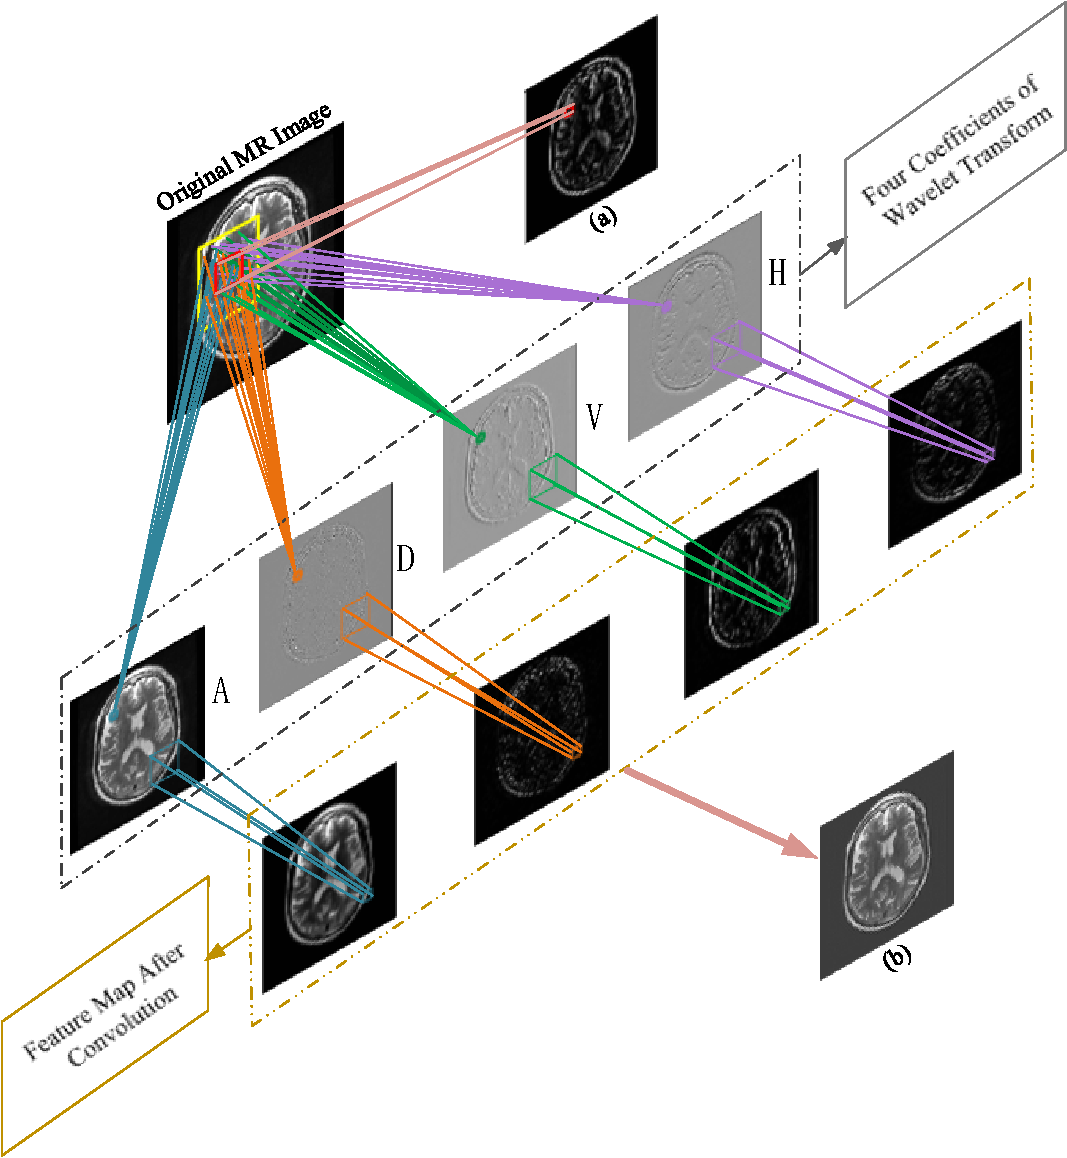
\includegraphics[width=0.8\linewidth]{figs/paper3nonLocalField2.pdf}
      \caption{卷积嵌入小波提取非局部感受野}\label{paper3nonLocalField2}
    \end{figure}
图\ref{paper3nonLocalField2}以一幅原始MRI为例的实现过程。根据新定义的卷积,首先通过小波变换生成四个系数分量(A:原始影像的近似表示,D:原始影像的对角边缘特征,V:垂直方向的奇异特征,H:水平方向的奇异特征)。然后对每个分量进行卷积,可得到四幅特征图。由于小波分解的四个系数表示不同的影像特征,因此在图\ref{paper3nonLocalField2}的原始MRI中,将它们堆叠后的区域用黄色框标记。初始卷积的局部感受野也用红框标记以供比较。根据小波变换理论,进一步的频域逐点更新将对小波变换中涉及的所有输入特征产生全局特征。当进行逆小波变换以获得最终的特征图(见图\ref{paper3nonLocalField2}(b))时,扩展的局部感受野进一步扩散到非局部感受野。并且,可以看到特征图影像非常接近原始影像,没有太多的信息损失。初始卷积的最终特征图如图\ref{paper3nonLocalField2}(a)所示,与原始影像有很大的不同,有很多信息丢失。

基于自定义的小波分解函数,本章提出了一个小波卷积单元,如图\ref{paper3framework}中黄色方块所示。它由四部分组成:编码器,WCU,解码器,全连接。WCU(wavelet convolution unit)是一个自定义的跨尺度信息提取模块,它利用小波分析和嵌入卷积来提取跨尺度信息。为了获得非局部的感受野,本章对单尺度小波分解系数进行卷积运算。此外,多尺度小波分解可以获得更全面的多尺度特征信息。此外,为了解决奇异点定位不准确的问题,本章将这些跨尺度特征融合到小波卷积单元中。本章的WCU如算法\ref{paper3algorithmWCU}所示。


\begin{algorithm}[ht]
\caption{Wavelet Convolution Unit}\label{paper3algorithmWCU}
\begin{algorithmic}[1]
\State {\textsc{WCU}}$~(X)$
\State \hspace{0.5cm}$W_s \gets$ SinScaT$~(X,~wave)$;
\State \hspace{0.5cm}$W_m \gets$ MulScaT$~(X,~wave)$;
\State \hspace{0.5cm}$W \gets$ Concatenate$~([W_s,~W_m],~1)$;
\State \hspace{0.5cm}$X_r \gets$ $\xi_{wav}~(W)$;
\State \hspace{0.5cm}\textbf{return} $X_r$;

\State \textbf{Function} {SinScaT}$~(X,~wave)$
\State \hspace{0.5cm}$C:\{c_i\}_{i=0}^3 \gets$ dwt$~(X,~wave)$;
\State \hspace{0.5cm}$\Hat{C}:\{\hat{c}_i\}_{i=0}^3 \gets$ $\xi_{wav}~({c}_0,~{c}_1,~{c}_2,~{c}_3)$;
\State \hspace{0.5cm}$\Gamma_s \gets$ idwt$~((\hat{c}_0,~\hat{c}_1,~\hat{c}_2,~\hat{c}_3),~wave)$;
\State \hspace{0.5cm}\textbf{return} $\Gamma_s$;

\State \textbf{Function} {MulScaT}$~(X,~wave)$
\State \hspace{0.5cm}$\Hat{C} \gets$  wavedec$~(X,~wave,~3)$;
\State \hspace{0.5cm}$\Gamma_{0,1} \gets$ idwt$~(\hat{c}_0,~\hat{c}_1,~wave)$;
\State \hspace{0.5cm}$\Gamma_{3,2} \gets$ idwt$~(\Gamma_{0,1},~\hat{c}_2,~wave)$;
\State \hspace{0.5cm}$\Gamma_m \gets$ idwt $~(\Gamma_{3,2},~\hat{c}_3,~wave)$;
\State \hspace{0.5cm}\textbf{return} $\Gamma_m$;
\end{algorithmic}
\label{alg1}
\end{algorithm}

\if 0
    \begin{figure}
      \centering
      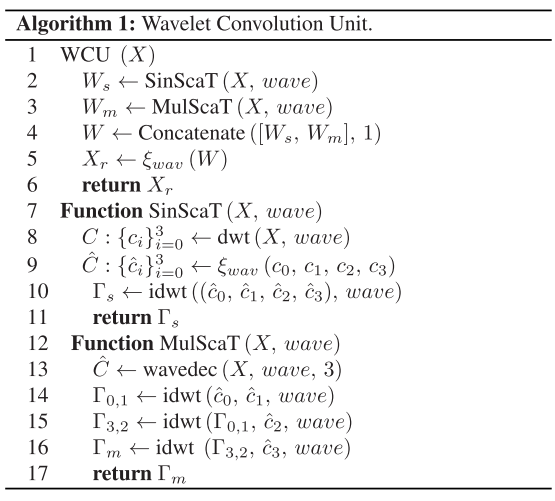
\includegraphics[width=0.75\linewidth]{figs/paper3Algorithm1WCU.png}
      \caption{WCU(Wavelet Convolution Unit)算法}\label{paper3algorithmWCU}
    \end{figure}
\fi
首先对影像进行单尺度分解,得到低频近似系数和三个(水平、垂直和对角)高频细节系数,并对每个系数应用$\xi$函数,然后对系数进行逆变换。在逆变换之前,先用$\xi$函数改变小波变换域的局部系数,可以选择性地扩大局部细节的分类,减少无用成分。同时将影像分解为三个尺度,根据不同尺度系数进行重构,得到变换后的特征图。最后,将两次重构的结果连接在一起,并再次应用$\xi$函数,以获得小波卷积单元的输出结果。在实验测试中,本章选择的小波基函数是Haar小波(一阶Daubechies小波),这是唯一直接适用于离散二维影像的不连续小波。Haar小波具有正交性和对称性。此外,在多尺度分解部分,本章设置了3尺度分解。在单尺度小波分解的卷积中,设置$size=1, stride=1, padding=0$在单尺度和多尺度组合的卷积中,设置$kernel size=3, stride=1, padding=1$。
    
    \begin{figure*}[t]
      \centering
      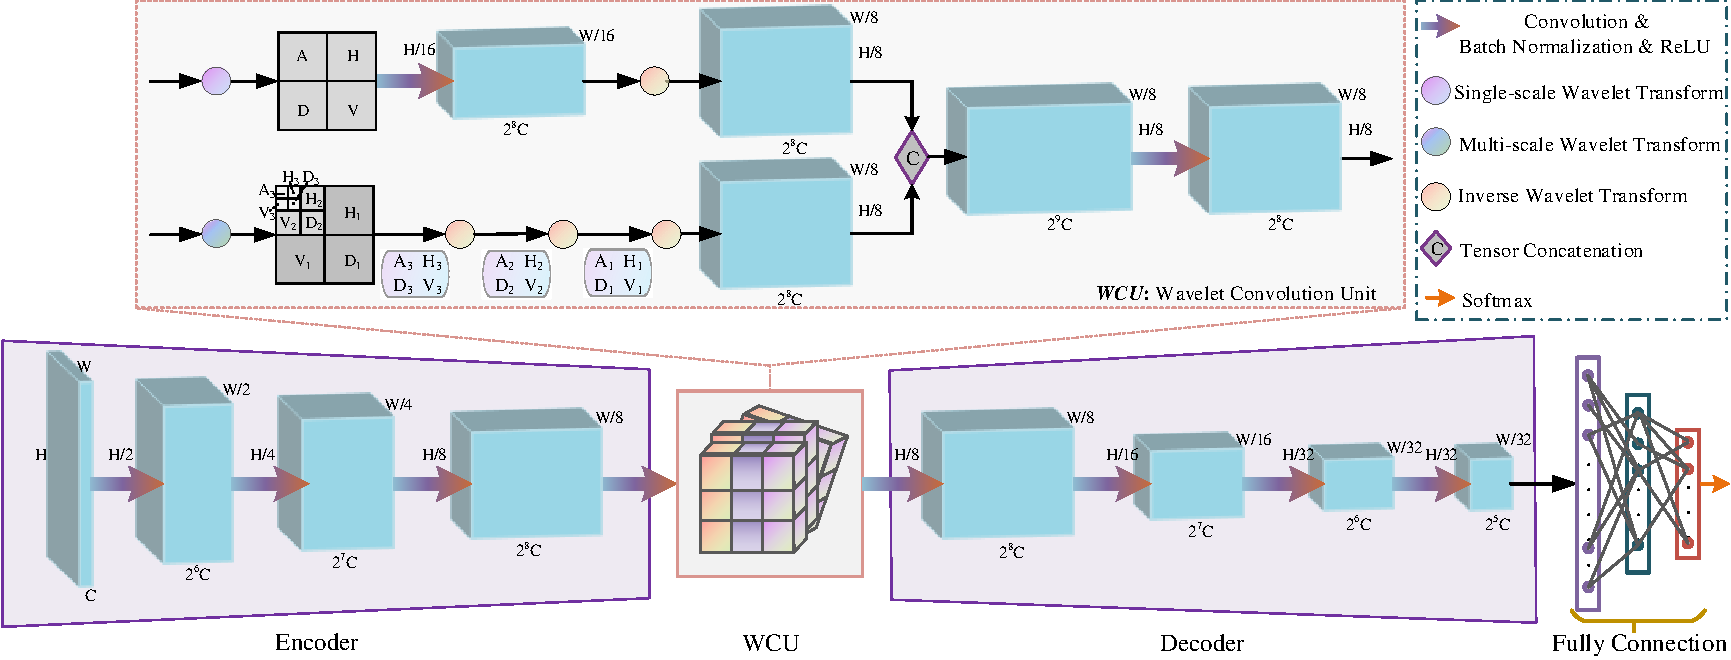
\includegraphics[width=0.9\linewidth]{figs/paper3framework.pdf}
      \caption{本节提出的小波卷积网络的框架图}\label{paper3framework}
    \end{figure*}


\subsection{细粒度多分类的网络结构}\label{paper3WCU-Net}
CNN作为深度学习中的一种典型网络结构,它由几层组成,包括但不限于卷积层、池化层、激活层和全连接层。本章方法的框架主要由四部分组成,包括编码,小波卷积单元,解码和全连接层,如图\ref{paper3framework}所示。为了有效地处理变长/短序列,使用编码和解码的思想。在编解码阶段,主要采用初级卷积运算来不断调整网络层的深度。在这两个过程中,使用了卷积层、BN和激活层的组合来提高网络模型的拟合能力。深度CNN的卷积层用于提取影像局部区域的尺度/位移不变特征。卷积层的主要好处是在同一特征图中共享权重,这减少了参数并导致模型的简单化。卷积层的不同层中的输入和输出通道的数量如图\ref{paper3framework}中蓝色框周围的值所示。在所有卷积层中,$kernel size=4, stride=2, padding=1$。卷积层后面是BN层,它本质上是一个归一化的网络层。

接着,将每个隐藏层神经元的输入逐步对接到非线性激活函数,最终归入该函数的值区间的极限饱和区域。将其设计为一般正态分布,其中,0为平均值,1为方差值。为了避免梯度消失,非线性函数被设计来处理输入特征。接下来是为模型引入激活层,以学习复杂的表示。为了提高收敛速度,本节中使用的激活函数(除了最终输出)是非线性激活函数ReLU。CNN的性能主要取决于层结构和滤波器集合,研究表明网络结构设计是提高CNN性能的有效途径\cite{liang2021cameranet}。本节基于小波的局部化和多分辨率特性,设计了一种小波卷积单元。最后一部分是全连接层。在前面的部分中处理的特征图已经变成了一个矢量,它不再是空间定位的。通过增加全连接层,可以发现卷积层中局部特征之间的非线性关系。本章使用了3层全连接,并通过softmax输出预测的类别。为了提高网络模型的泛化能力,在全连接前后采用了dropout方法,并将系数设置为0.5。在训练过程中,本章使用经典的交叉熵损失函数计算真实的标签和预测输出之间的损失。


\subsection{临床特征驱动型辅助分类}\label{paper3WCUNetClassify}

\subsubsection{临床特征驱动的脑影像数据}
众所周知,数据预处理一直是深度学习模型的重要步骤,尤其是在医学领域。DTI是MRI的一种特殊表现形式,是一种能有效观察和追踪白色纤维束的无创性方法。MRI主要用于AD和其他症状的诊断。一般来说,DTI能更好地反映脑部疾病的特征,有利于诊断。

在三维视图中,用对称矩阵的概念量化扩散各向异性的信号数据,定义为$D$,如等式(\ref{paper3dti})。其中,$D_{xx}$、 $D_{yy}$、 $D_{zz}$是沿着空间直角坐标系的$x$、$y$、$z$轴三个相互正交方向上传播的弥散系数。DTI表现为一个3$\times$3对称正定矩阵,它包含三个特征值($\lambda_{1}$, $\lambda_{2}$, $\lambda_{3}$)和相关的特征向量$V=(v_1, v_2, v_3)^T$。这3个特征向量分别指示了水分子扩散的三个主要方向,而与之对应的特征值则体现了水分子在这三个方向上的弥散强度。

\begin{equation}\label{paper3dti}
\begin{aligned}
D &=\left(\begin{array}{lll}
D_{xx} & D_{xy} & D_{xz} \\
D_{xy} & D_{yy} & D_{yz} \\
D_{xz} & D_{yz} & D_{zz}
\end{array}\right) & = V^T\left(\begin{array}{ccc}
\lambda_{1} & 0 & 0 \\
0 & \lambda_{2} & 0 \\
0 & 0 & \lambda_{3}
\end{array}\right)V.
\end{aligned}
\end{equation}

在本章的方法中,使用DTI的FA和MD指标($Ind_{FA}, Ind_{MD}$分别由式(\ref{paper3FA})和(\ref{paper3MD})表达),这两个指标可以使用FSL软件或脚本对DTI数据进行预处理获得。如图\ref{paper34classify}中黄色背景的方块所示。MD影像在第一行,第二行是FA影像。FA的值与白质内部髓鞘的完整性、纤维束的密集程度以及纤维排列的平行性呈正相关关系。因此,FA影像对脑内白质纤维结构的观察最为清晰,灰质边界明显。$Ind_{FA}$的计算公式如(\ref{paper3FA})所示。其中,$\bar{\lambda}$ 是三个特征值的平均值。MD反映了分子的整体扩散水平和阻力。MD仅反映了扩散的整体程度,而不涉及扩散的具体方向。$Ind_{MD}$越大,组织中包含的游离水分子越多。$Ind_{MD}$的计算公式如(\ref{paper3MD})所示。$Tr(D)$是$D$的迹,它是一个矩阵不变量。

 \begin{equation}\label{paper3FA}
Ind_{FA}=\sqrt{\frac{\sum_{i=1}^{3}3\left(\lambda_{i}-\bar{\lambda}\right)^{2}}{\sum_{i=1}^{3}2\lambda_{i}^{2}}},
\end{equation}
\begin{equation}\label{paper3MD}
Ind_{MD}=Tr(D)/3=\left(D_{xx}+D_{yy}+D_{zz}\right)/{3}.
\end{equation}


\subsubsection{细粒度与多分类的技术路线}\label{4.3.3.2}
本节建立了一个新的框架,通过WCU-Net实现AD的细粒度和多分类。对于二、三和四分类框架通用,在实验装置中,只有它们的输入和输出不同。如图\ref{paper34classify}所示,该框架包括三个部分:数据输入,编码器、WCU、解码器、FC和激活函数的网络架构,以及类别预测的输出。在第一部分中,对DTI数据进行了预处理。FSL(https://fsl.fmrib.ox.ac.UK/fsl/fslwiki/Fsl Installation/Linux)工具对原始DTI数据进行b0影像提取、剥脑、涡流校正、张量计算等预处理操作。从所获得的张量指数中选择FA和MD作为输入的数据。在第二部分中,依次输入4个类别(AD,NC,EMCI,LMCI)的FA和MD,并分别通过编码器,WCU,解码器,FC和激活函数(Softmax)。在这一部分中,主要对WCU中的流程进行了扩展和展示。WCU采用自定义的小波卷积单元,结合单尺度小波分解和多尺度小波分解的特点,获得完整的跨尺度特性。最后一部分是网络的预测输出,其将概率分布转换为标签数据。最终的预测类别取决于具有最高概率的类别。
    \begin{figure*}[ht]
      \centering
      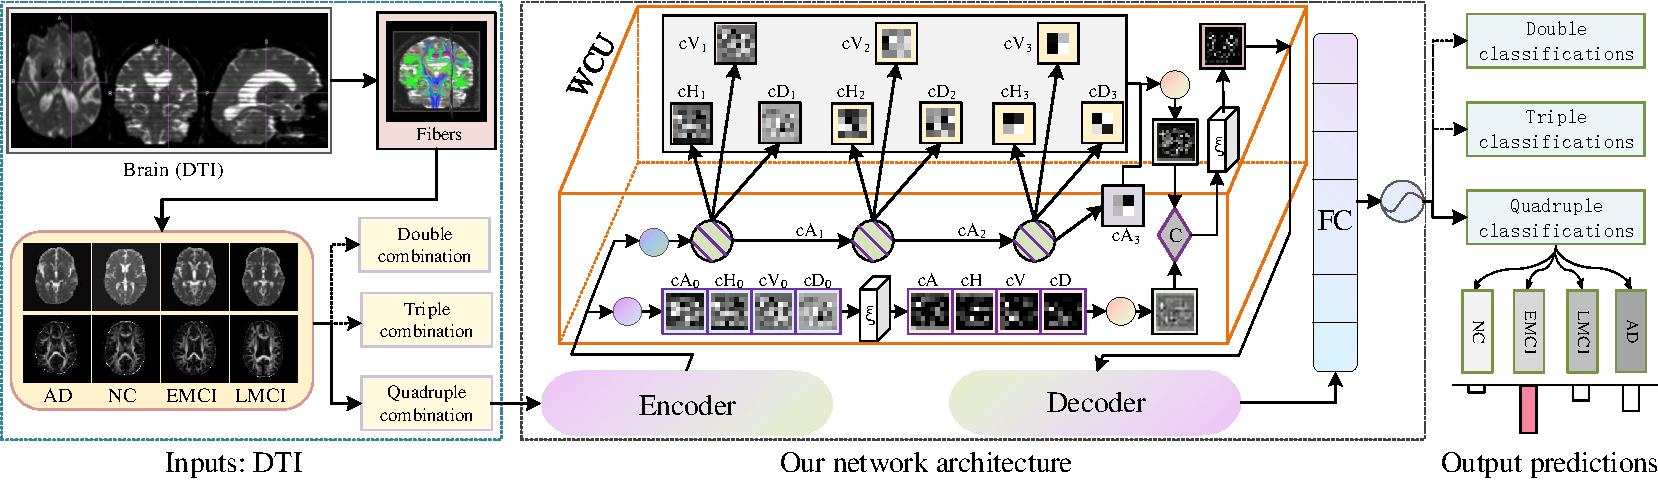
\includegraphics[width=0.9\linewidth]{figs/paper34classify.pdf}
      \caption{WCU-Net应用于细粒度多分类任务中的具体步骤} \label{paper34classify}
    \end{figure*}


%\subsubsection{预训练模型参与应用的分析}
CNN是深度智能系统中最常用于检测AD的网络,一些研究倾向于设计CNN的结构\cite{bringas2020alzheimer}。经典的网络结构,如ResNet,DenseNet,SqueezeNet,Inception,AlexNet,VGGNet和GoogLeNet,已成功应用于影像分类任务\cite{ananda2021classification},这有助于权重初始化过程。在本节中,利用这7个经典的网络模型初始化本章提出的网络结构权重。表\ref{paper3withPretrained}列出了WCU-Net与预训练CNN的分类准确度,其中,D-1: AD vs. NC, D-4: AD vs. EMCI, D-5: AD vs. LMCI, D-6: NC vs. EMCI, D-7: NC vs. LMCI, D-8: EMCI vs. LMCI, T-2: AD vs. EMCI vs. LMCI, T-3: NC vs. EMCI vs. LMCI, QC: AD vs. NC vs. EMCI vs. LMCI),2-9列的每一列表示不同的网络模型参与的应用(Net\_1: ResNet101, Net\_2: DenseNet161, Net\_3: SqueezeNet1\_1, Net\_4: Inception\_v3, Net\_5: AlexNet, Net\_6: VGG13, Net\_7: GoogLeNet, Net\_8:w/o pretrained CNNs。在权重初始化过程中是否采用预训练CNNs模型的分类准确率也列在最后一列以供比较。从表\ref{paper3withPretrained}可以看出,每个预训练模型都能在一定程度上提高2-4种组合分类的准确率,在第2-8列用红色或蓝色值标记。特别是对于细粒度的NC vs. EMCI和NC vs. LMCI二分类,预训练的效果明显。总之,九种组合分类的最高准确度值分别达到0.9920,0.9730,0.9611,0.9870,0.9611,0.9900,0.9636和0.9379,其中AD与NC,AD与EMCI和AD与LMCI与EMCI与NC的最佳分类准确度由WCU-Net得到,无预训练CNNs模型参与。而在本节中,所提出的方法则是使用未经预训练网络初始化参数的WCU-Net,并获得的结果与现有的AD分类方法进行比较。

\begin{table}[ht]
 \centering
\caption{权重初始化过程中是否采用预训练模型的精度比较}
%\small
\begin{tabular}{ccccccccc}
\toprule
Class   &  Net\_1 &  Net\_2   &  Net\_3 &Net\_4   & Net\_5  & Net\_6  &  Net\_7   &\textbf{Net\_8}    \\ \midrule
D-1 & 0.9840 & 0.9890 & 0.9790  & 0.9710 & 0.9701 & 0.9850 & 0.9890 &\textcolor{red}{{0.9920}}  \\
D-4 & 0.9630 & 0.9550 & 0.9690 & 0.9670  & 0.9500 & 0.9480 & 0.9680 &\textcolor{red}{{0.9730}}  \\
D-5 & 0.9533 & 0.9556 & 0.9533 & 0.9511 & 0.9478 & \textcolor{red}{{0.9611}} & 0.9522 & 0.9578    \\
D-6  & \textcolor{green}{{0.9750}}           & \textcolor{green}{{0.9720}}
& \textcolor{green}{{0.9650}}
& \textcolor{green}{{0.9710}}
& \textcolor{green}{{0.9690}}
& \textcolor{red}{{0.9870}}
& \textcolor{green}{{0.9700}}
& 0.9500    \\
D-7 & \textcolor{red}{{0.9611}}
& \textcolor{green}{{0.9533}}
& \textcolor{green}{{0.9456}}
& \textcolor{green}{{0.9489}}
& \textcolor{green}{{0.9567}}
& 0.9089
& \textcolor{green}{{0.9590}}
& 0.9400    \\
D-8
& \textcolor{green}{{0.9800}}
& \textcolor{green}{{0.9800}}
& 0.9722
& \textcolor{green}{{0.9833}}
& 0.9644
& 0.9778
& \textcolor{red}{{0.9900}}
& 0.9789\\
T-2
& 0.9350
& \textcolor{green}{{0.9586}}
& 0.9490
& 0.9521
& \textcolor{green}{{0.9600}}
& \textcolor{green}{{0.9586}}
& \textcolor{red}{{0.9636}}
& 0.9571\\
T-3
& 0.9257
& 0.9243
& 0.9464
& \textcolor{red}{{0.9833}}
& 0.9193
& 0.9407
& 0.9429
& 0.9507
\\
QC
& 0.9353
& 0.9168
& 0.9284
& 0.9068
& 0.9358
& 0.9337
& 0.9053
& \textcolor{red}{{0.9379}}
\\ \bottomrule
\end{tabular}
\label{paper3withPretrained}
\end{table}


\section{细粒度多分类的实验}\label{chapter4.4}
\subsection{实验验证的数据说明}
本节中使用的数据来自ADNI(www.adni-info.org)。由于每个类别的数据量不相等,并且数据的总数不足以训练深度学习模型,因此使用数据扩大来增加每个少数类别的样本数量。另外,医学影像可视化后是灰度影像,为了不对影像造成较大的改变,数据增强方法主要是通过加入随机噪声和亮度进行扩大。为了增加数据的大小,本章将使用数据增强来扩展所获得的数据。数据增强的方法与文献\cite{Fangmeie2022}一致,数据增强后的情况见表\ref{paper3sourceData}。

\begin{table}[ht]
\centering
\caption{增强前后的数据集详情}\label{paper3sourceData}
\begin{tabular}{ccccc}
\hline
\normalsize
Diagnosis      & \multicolumn{1}{c}{AD}      & \multicolumn{1}{c}{EMCI}      & \multicolumn{1}{c}{LMCI}     & \multicolumn{1}{c}{NC}        \\ \hline
Age            & \multicolumn{1}{c}{75.23}   & \multicolumn{1}{c}{73.95}     & \multicolumn{1}{c}{73.45}    & \multicolumn{1}{c}{74.52}     \\
Gender(M/F)   & \multicolumn{1}{c}{99 / 54} & \multicolumn{1}{c}{225 / 138} & \multicolumn{1}{c}{108 / 59} & \multicolumn{1}{c}{110 / 109} \\
Subjects       & \multicolumn{1}{c}{153}     & \multicolumn{1}{c}{363}       & \multicolumn{1}{c}{167}      & \multicolumn{1}{c}{219}       \\
MMSE           & \multicolumn{1}{c}{18-27}   & \multicolumn{1}{c}{24-30}     & \multicolumn{1}{c}{24-30}    & \multicolumn{1}{c}{25-30}     \\ \hline\hline
Train data & \multicolumn{1}{c}{9273}    & \multicolumn{1}{c}{9748}      & \multicolumn{1}{c}{10154}    & \multicolumn{1}{c}{10113}     \\
Valid data & \multicolumn{1}{c}{2100}    & \multicolumn{1}{c}{2088}      & \multicolumn{1}{c}{2100}     & \multicolumn{1}{c}{2200}      \\
Test data   & \multicolumn{1}{c}{500}     & \multicolumn{1}{c}{400}       & \multicolumn{1}{c}{500}      & \multicolumn{1}{c}{500}       \\ \hline
\end{tabular}
\end{table}

DTI是MRI的一种特殊形式,但其获取比MRI困难。DTI可以捕捉脑内的白色物质束和灰质束,并通过测量活体组织内水分子的扩散来工作。由于扩散张量是一个对称的$3 \times3$矩阵,它可以用它的特征值($\lambda_{i}$)和特征向量($V_{i}$)来描述,然后使用特征值和特征向量来处理标量指数。两个主要的扩散指数(FA和MD)是基于本征值和代表的扩散过程的幅度。年龄是AD的主要危险因素,因此选择年龄在73-76岁之间且认知功能评分差异显著的人群(AD:18-27,EMCI/LMCI:24-30,NC:25-30)进行研究分析。所下载的数据集来自902个样本,分为四类:153个AD患者,167个LMCI,363个EMCI和219个NC。选择DTI数据集作为模型的训练集、验证集和测试集,数量如表\ref{paper3sourceData}所示。

\subsection{实验验证的参数说明}
在网络训练过程中,影像的大小为128 × 128。在训练过程中,初始学习率为0.001,40个epoch,批量大小为32,使用批量归一化。优化函数是SGD,动量的值为0.85。此外,实施了一种动态调整的学习率策略,每隔8个训练周期将学习率降低至初始值的10\%。本章使用Python 3.8.12和Pytorch 1.10.2版本,CUDA版本为10.2,系统为Tesla T4 16 G RAM 64 GNU/Linux x86。

\subsection{早期细粒度分类应用}
临床研究表明,AD的细粒度分型具有重要意义。关于AD的分类有很多研究,然而,大多数现有的方法局限于粗粒度的二分类,即,AD vs. NC、AD vs. MCI和MCI vs. NC。一些方法实现了粗粒度的三分类,即,AD与NC与MCI分类。近年来,一些学者对MCI进行了进一步的细粒度分类。早期很少有学者利用DTI数据做细粒度的二分类\cite{prasad2015brain, 2020Convolutional},其较高的准确率为0.81。一些学者使用MRI数据对AD进行了细粒度的四分类。Ashburner和Friston\cite{ashburner2000voxel}、Zhang等人\cite{zhang2016detecting}和Liu等人\cite{liu2018joint}提出应用于AD细粒度四分类并使用MRI数据的方法,但准确性较低。也有一些方法使用MRI数据应用于三分类和四分类,可以获得更好的性能。例如,在\cite{sorensen2018ensemble}中,三分类准确率可以达到68.8\%,四分类准确率可以达到59.1\%。然而,三分类是AD vs NC vs(EMCI+LMEC),这与传统的粗粒度三分类相似。在文献\cite{dimitriadis2018random}中四分类的准确率可达61.9\%。Basaia等\cite{2018Automated}提出了基于CNN的MRI数据MCI细粒度分类方法,实现了AD、LMCI、EMCI、NC六种组合双分类。Fang等人\cite{Fangmeie2022}提出了一种通过二次迁移学习的细粒度方法,提高了5种细粒度二分类的准确性。目前,De和Chowdhury\cite{de2021dti}实现了细粒度的四分类,精度为0.926。

     \begin{figure*}[ht]
      \centering
      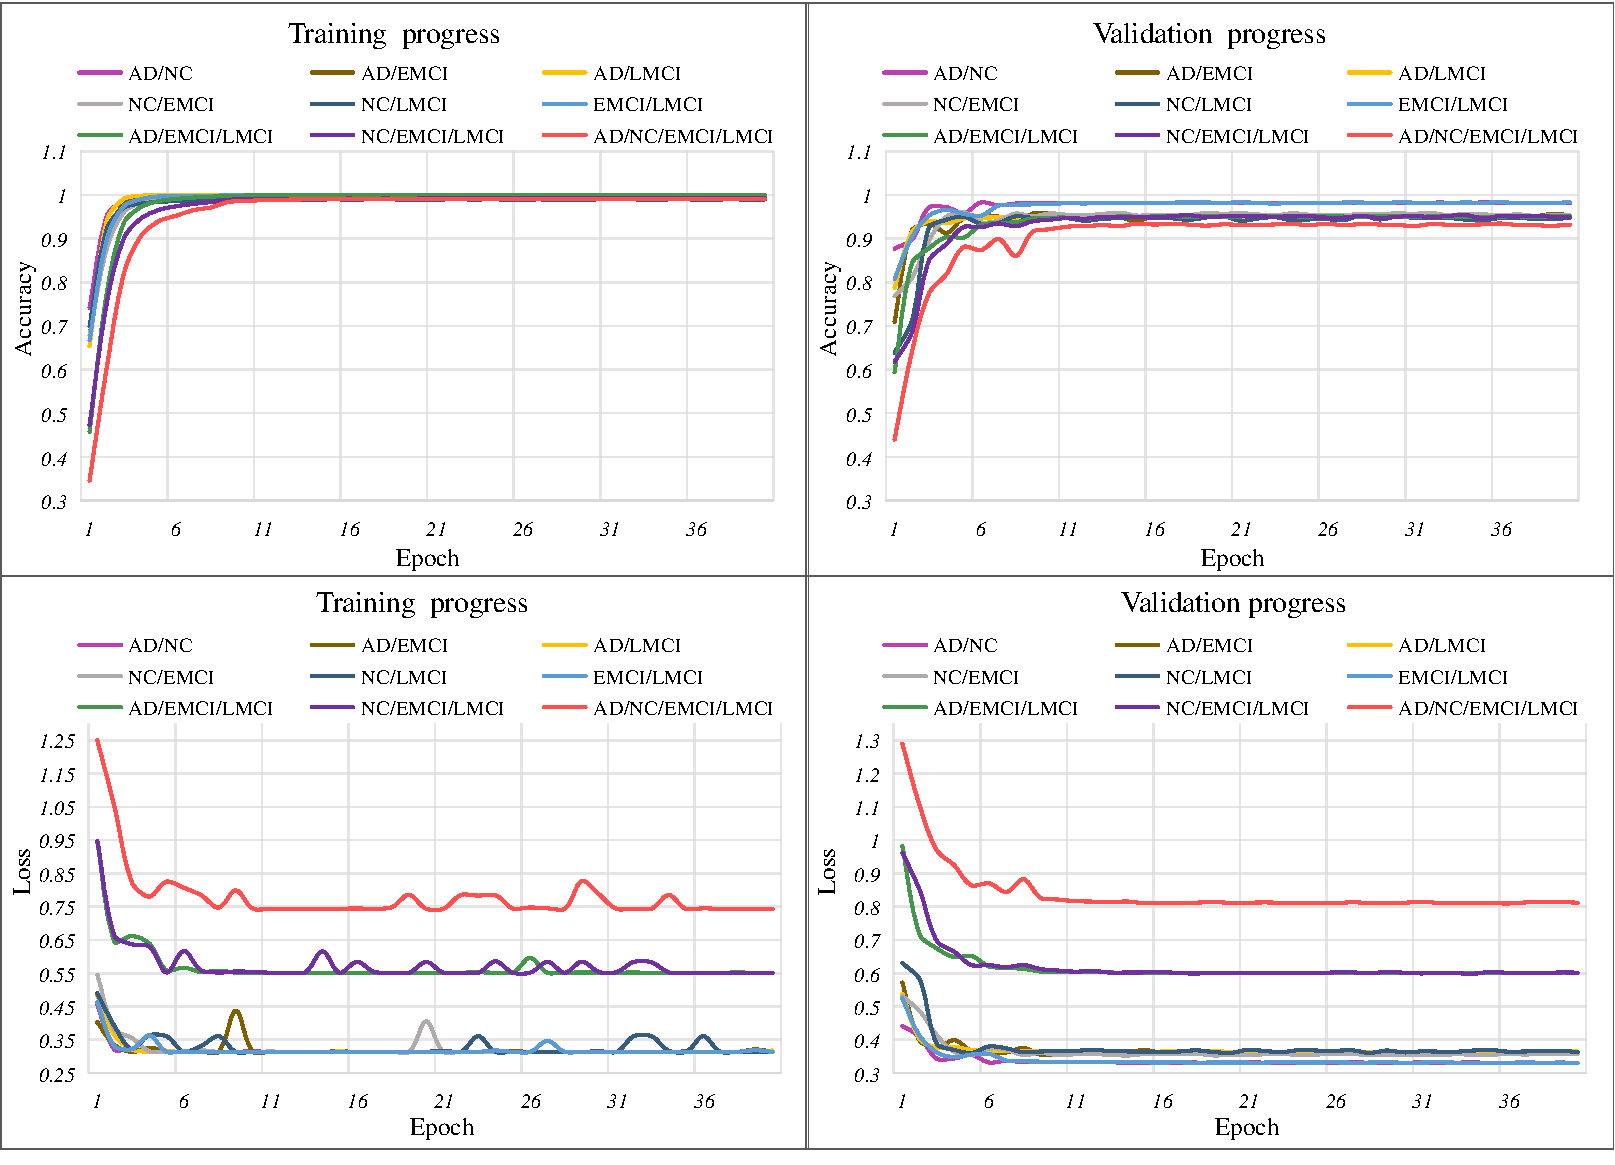
\includegraphics[width=0.9\linewidth]{figs/paper3lossandaccuracy.pdf}
      \caption{准确度曲线和损失曲线}\label{paper3curves}
    \end{figure*}
    
在本节中,为了便于尽可能准确地诊断AD分类,展开了12种组合分类,包括4种粗粒度分类和8种细粒度分类,如表\ref{paper3accuracy1}和\ref{paper3fine_classify}的所示。本章提出的方法是首次出现两种细粒度的三分类(AD vs. LMCI vs. EMCI和NC vs. LMCI vs. EMCI)。
表\ref{paper3fine_classify}列出了本章提出的方法对AD与NC分类以及8种粒度多分类的准确性。为便于比较,表\ref{paper3fine_classify}还列出了现有细粒度分类方法的准确性。可以观察到,对于实现的6种二分类,本章提出的方法的准确性比现有的方法\cite{2018Automated,Fangmeie2022}要好得多。对于细粒度的四分类,本章提出的方法准确率为0.9379,也比\cite{de2021dti}提高了1.19\%,首次实现了细粒度的三分类,其中AD vs. EMCI vs. LMCI、NC vs. EMCI vs. LMCI的准确度分别达到0.9571和0.9507。

图\ref{paper3curves}中的第一行显示了在没有预训练的网络模型作为初始化权重参数的情况下,所提出的方法的预测精度曲线分布,并且在训练阶段和验证阶段之间的分布存在一定的偏差。在训练过程中,准确率曲线没有波动,并且随着训练时期的增加,在不同分类组合中的准确率更接近于1。在验证过程中,1-8轮出现了小范围的振荡,但总体上升趋势是正确的。在验证过程中,参数不断更新。随着轮数的增加,AD vs. NC和EMCI vs. LMCI分类的准确率接近1,四分类的准确率稍低,但也在0.9-1之间。在其他数据组合分类的情况下,精度也稳定在第11轮。图\ref{paper3curves}中的第二行显示了训练和验证阶段的损失曲线。二分类的损失较小,而四分类的损失相对较大。而训练和验证过程中的损失明显减少,并趋于稳定。因此,表明本节提出的网络模型具有良好的泛化性能。

    \begin{figure*}[ht]
      \centering
      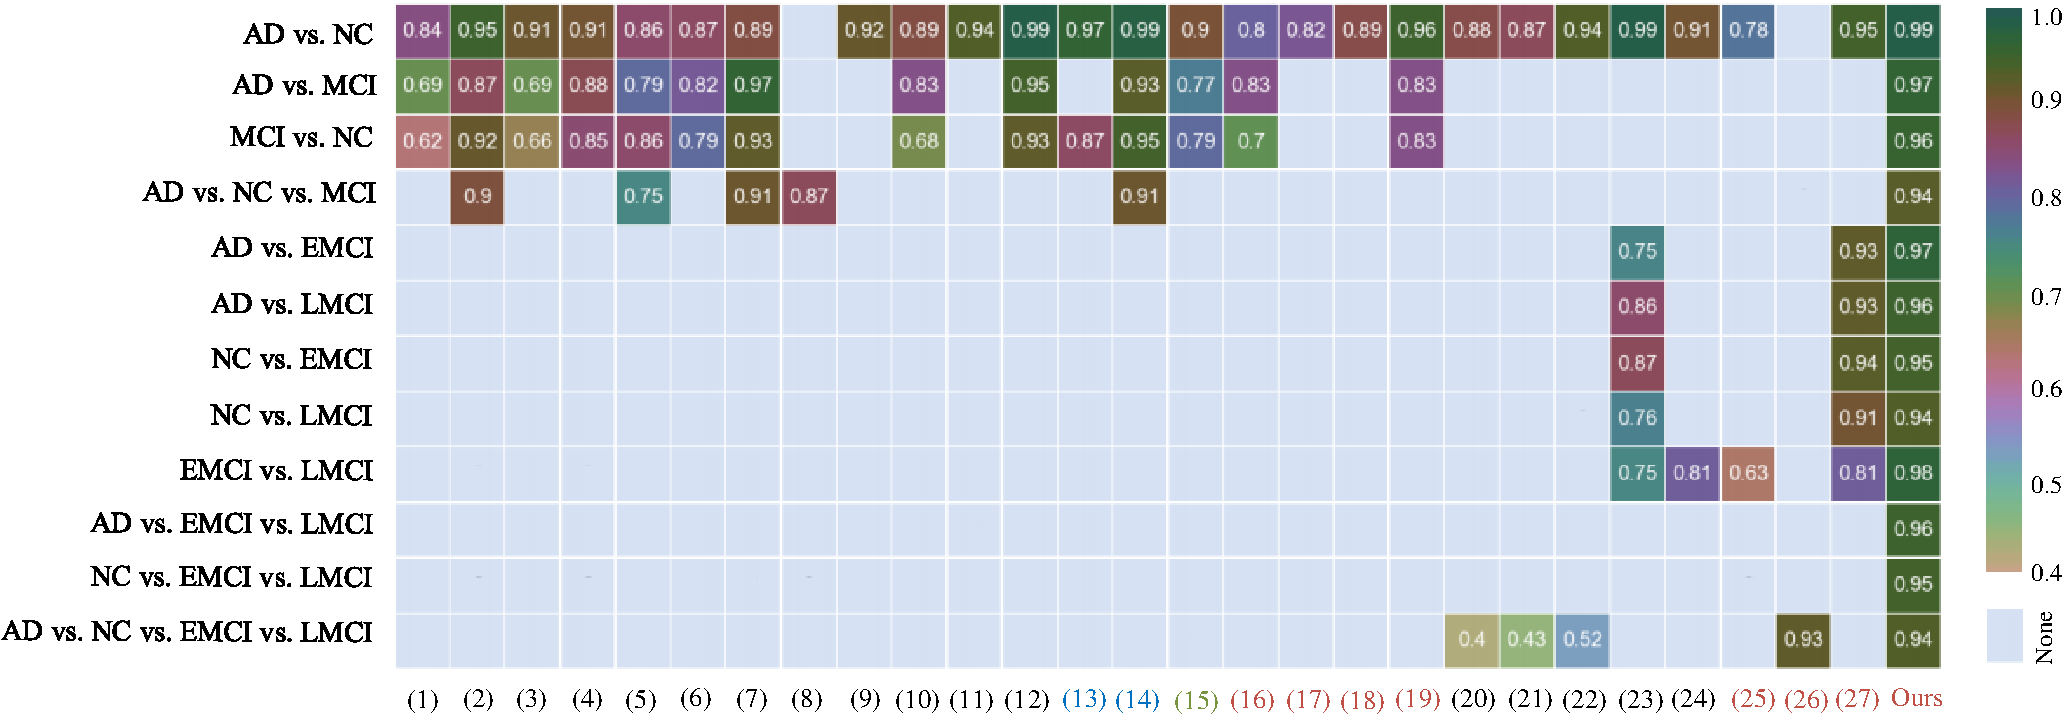
\includegraphics[width=0.9\linewidth]{figs/paper3rlt20230306-2.pdf}
      \caption{各种粗粒度和细粒度AD分类方法精度比较的热力图}\label{paper3heatmap}
    \end{figure*}
    
\subsection{多类别分类应用分析}
图\ref{paper3heatmap}显示了本文所涉及的所有粗粒度和细粒度AD分类的准确性比较的热力图。图中的小矩阵单元颜色越深,其相应方法的准确度越高。淡蓝色单元格表示没有相应的分类工作。大面积的浅蓝色单元表明,大多数现有的方法只关注于少数组合分类。但本章提出的方法实现了所有12种分类,对于所有细粒度分类都具有较高精度,为以后该领域的研究工作提供了完整的参考。图中横轴上颜色相同的数字表示这些方法使用的数据模态是相同的。红色、蓝色、绿色和黑色分别对应于DTI、MRI+PET、MRI+DTI和MRI。(1)-(27)列分别指下列参考文献中提出的不同方法:Ben Ahmed et al. \cite{ahmed2015alzheimer}, Payan and Montana \cite{payan2015predicting}, Aderghal et al. \cite{aderghal2017classification}, Yang et al. \cite{yang2017active}, Xiao et al. \cite{xiao2017brain}, Madusanka et al. \cite{madusanka2019alzheimer}, Bi et al. \cite{bi2020computer}, Duc et al. \cite{duc20203d}, Xing et al. \cite{xing2020dynamic}, Pan et al. \cite{pan2020early}, Ebrahimi and Luo \cite{ebrahimi2021convolutional}, Liu et al. \cite{liu2022diagnosis}, Lei et al. \cite{lei2016discriminative}, Vu et al. \cite{vu2018non}, Ben Ahmed et al. \cite{ahmed2017recognition}, Ebadi et al. \cite{ebadi2017ensemble}, Qu et al. \cite{qu2021ai4ad}, Lella et al. \cite{lella2021ensemble}, Bigham et al. \cite{bigham2022features}, Ashburner and Friston \cite{ashburner2000voxel}, Zhang et al. \cite{zhang2016detecting}, Liu et al. \cite{liu2018joint}, Basaia et al. \cite{2018Automated}, Wen et al. \cite{2020Convolutional}, Prasad et al. \cite{prasad2015brain}, De and Chowdhury \cite{de2021dti}, Fang et al. \cite{Fangmeie2022}。从这张热图中,可以得出以下结论:
\begin{itemize}
    \item 大多数方法只能实现粗粒度的分类。一些方法实现了一种或几种细粒度分类。本章的方法实现了所有12种的组合分类,而且只有本章的方法实现了细粒度的三分类。
    \item 大多数方法对于不同类别组合的精度不稳定,甚至存在许多精度小于0.70。本章的方法实现了稳定的分类且精度高于0.935的有12种组合分类。

\end{itemize}
    
  \begin{figure}[ht]
      \centering
      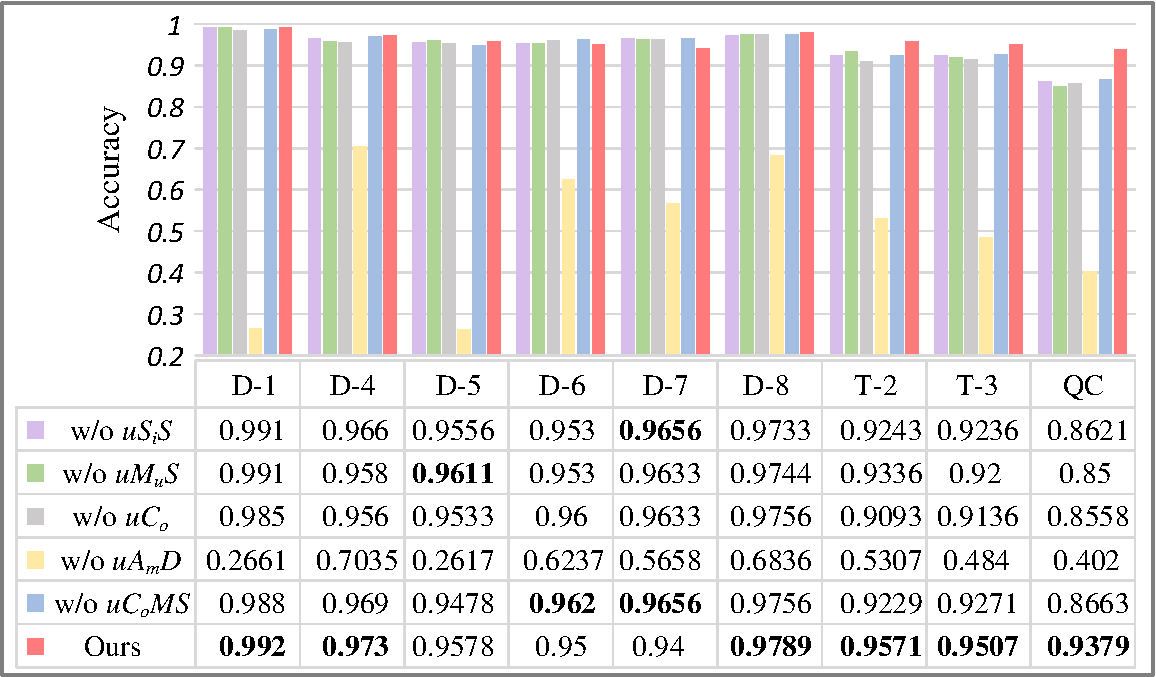
\includegraphics[width=0.9\linewidth]{figs/paper3ablation4.pdf}
      \caption{本章提出的方法的消融实验}\label{paper3ablation}
    \end{figure}  
关于AD分类的研究工作似乎很多,但他们通常专注于不同的数据模态和类别的组合,各种方法之间的可比性不是很强。本章方法实现了所有12种粗粒度和细粒度分类,具有较高的准确率,为后续基于DTI数据的AD分类研究提供了一个合适的参考标准。不过,有一点需要特别说明。在本章中,主要集中在DL方法的准确性,但忽略了神经科学的部分,潜在的目标对的ROI可以关联到AD的不同阶段。实际上,这对于基于神经科学的疾病研究和基于深度学习方法的智能辅助诊断的可解释性非常重要。在未来的研究中,将神经科学与人工智能方法更深入地结合将是一个有意义的研究方向。

\subsection{细粒度多分类的消融实验}

如第\ref{chapter4:WCU-net}节所述,本章的方法的最佳性能主要取决于单尺度小波分解($uS_{i}S$)、多尺度小波变换($uM_{u}S$)、$\xi$函数运算($uC_{o}$)和数据扩增$uA_{m}D$。为了进一步证明这四个部分的有效性,本章设计了五组方法进行消融实验,即,缺少$uS_{i}S$、缺少$uM_{u}S$、缺少$uC_{o}$、缺少$ uA_{m}D$和缺少$uC_{o}MS$(缺少$uM_{u}S$和$uC_{o}$)。所有的实验结果都显示在图\ref{paper3ablation}中,与本章的方法进行比较。表格中的每行表示的是不同的方法,每列代表不同的组合分类,各组合同章节\ref{4.3.3.2}定义的相同。从图\ref{paper3ablation}可以发现,数据扩增至关重要,其他部分对于细粒度分类也很重要。特别是在细粒度的四分类中,各组件的结合使用,分类精度有了明显的提高。



\section{本章小结}\label{chapter4.5}
本章提出了一种新的网络WCU-Net,它在小波卷积单元中结合了单尺度和多尺度变换。该策略不仅获得了非局部感受野,而且实现了跨尺度信息融合。然后将WCU-Net成功地应用于AD细粒度和多分类中,并达到SOTA精度。细粒度分类对于认知障碍的准确诊断和正确治疗具有重要意义。细粒度分类特别是细粒度的四分类准确率还有待进一步提高。后续将会尝试在AD的更多分期中应用WCU-Net,以及基于医学影像的不同性质疾病的分类,并进行更多研究。